%
% File eacl2017.tex
%
%% Based on the style files for ACL-2016
%% Based on the style files for ACL-2015, with some improvements
%%  taken from the NAACL-2016 style
%% Based on the style files for ACL-2014, which were, in turn,
%% Based on the style files for ACL-2013, which were, in turn,
%% Based on the style files for ACL-2012, which were, in turn,
%% based on the style files for ACL-2011, which were, in turn, 
%% based on the style files for ACL-2010, which were, in turn, 
%% based on the style files for ACL-IJCNLP-2009, which were, in turn,
%% based on the style files for EACL-2009 and IJCNLP-2008...

%% Based on the style files for EACL 2006 by 
%%e.agirre@ehu.es or Sergi.Balari@uab.es
%% and that of ACL 08 by Joakim Nivre and Noah Smith

\documentclass[11pt]{article}
\usepackage{eacl2017}
\usepackage{times}
\usepackage{url}
\usepackage{latexsym}
\usepackage{graphicx}

\eaclfinalcopy % Uncomment this line for the final submission
%\def\eaclpaperid{***} %  Enter the acl Paper ID here

%\setlength\titlebox{5cm}
% You can expand the titlebox if you need extra space
% to show all the authors. Please do not make the titlebox
% smaller than 5cm (the original size); we will check this
% in the camera-ready version and ask you to change it back.

\newcommand\BibTeX{B{\sc ib}\TeX}

\title{OpenNMT: Open-Source Toolkit for Neural Machine Translation}

\author{Guillaume Klein$^\dagger$, Yoon Kim$^*$, Yuntian Deng$^*$, Jean Senellart$^\dagger$, Alexander M. Rush$^*$ \\ Harvard University$^*$, Systran $^\dagger$}

\date{}

\begin{document}
\maketitle
\begin{abstract}

  We describe an open-source toolkit for neural machine translation
  that supports research development of sequence-to-sequence models.
  The toolkit prioritizes simplicity, modularity, and efficiency to
  make it reasonable for researchers to experiment with variants of
  neural machine translation that explore different feature
  representations, model architectures, and source (multi)-modalities,
  while maintaining competitive performance and tractable training
  requirements. The toolkit consists of modeling and decoding support,
  as well as detailed pedagogical documentation about the underlying
  methodologies.

\end{abstract}

\section{Introduction}


Neural machine translation (NMT) is a new methodology for machine
translation \cite{}, that has shown remarkable gains particularly in
terms of human evaluation. Originally popularized by the work of
\cite{} and expanded upon by \cite{}. Over the last year the systems
have been further refined and developed by work such as \cite{}.

In this work we describe a new open-source toolkit for developing
neural machine translation systems, known as \textit{OpenNMT}. The
system is motivated by frameworks, such as Moses and CDec developed
for statistical machine translation (SMT). These toolkits aim to
provide a shared frameworks for developing and comparing open-source
SMT systems that are complete and flexible enough for research
development, while at the same time being efficient and accurate
enough to be used production contexts. 


Currently there are several existing NMT systems. Including Google NMT
\cite{}, ... Several of these systems are proprietary. Several others
are mainly research system such as seq2seq-attn. Perhaps most similar
to OpenNMT is the NeMaTus system \cite{}, based on the system of \cite{}
which aims to provide the same type of feature set as OpenNMT, using a
different underlying neural network toolkit.

In developing OpenNMT we prioritized three different factors, which
are described in this technical report: (1) Our top priority was
training and decoding speed. NMT systems are notoriously slow to
train, often requiring weeks of training time on the latest GPU
hardware and significant test resources. We targeted this issue by
implementing multi-GPU training, using aggressive memory sharing, and
developing a specialized CPU decoder. (2) Our second priority was system
modularity and teachibility. We intend OpenNMT as a living research
system, and so the codebase was developed to provide a
self-documenting overview of NMT. We discuss how this approach allowed
us to add factored models \cite{} to the system. (3) Finally NMT is a very 
quick moving research area, and we would like the system to support 
new research areas as they develop. To demonstrate this approach we 
abstracted out the core of OpenNMT as a library, and describe the case 
study of using OpenNMT for image-to-text translation. 

This report describes the background for NMT, the main aspects of system development, and the preliminary results from using the system in practice.  


\section{Background}

Neural machine translation has now been extensively described in many
excellent papers and tutorials \cite{}, which we briefly summarize.
NMT systems take a conditional language modeling view of translation
(as opposed to the noisy channel view of SMT systems). This means they
model the probability of a target sentence $w_{1:T}$ given a source
sentence $x$ as
$p(w_{1:T}| x) = \prod_{1}^T p(w_t| w_{1:t-1}, x; \theta)$. This
distribution is modeled using an attention-based encoder-decoder
architecture \cite{}. In particular a source encoder recurrent neural network
(RNN) maps each source word to a word vector, and processes these to a
sequence of hidden vectors $\mathbf{h}_1, \ldots, \mathbf{h}_S$. To produce the language model probability a target decoder RNN, combines a representation of previously generated words ($w_1, ... w_{t-1}$) with these source hidden vectors and a softmax layer to produce $ p(w_t| w_{1:t-1}, x; \theta)$. The source hidden vectors are utilized through an attention layer, a type of pooling that weights each source word relative to its expected contribution to the target prediction.
The complete model is trained end-to-end to minimize the negative log-likelihood of the training corpus. 


In practice, there are also several important details that contribute to model effectiveness. (a) It is important to use a gated RNN such as an LSTM \cite{} or GRU \cite{} which help the model learn long-term features. (b) Translation requires relatively large, stacked RNNs, which consist of several layers (2-16) of RNN at each time step \cite{}. (c) Input feeding, where the previous attention vector is fed back into the input as well as the predicted word, has been shown to be quite helpful for machine translation \cite{}. OpenNMT provides command-line support for each of these options.



\begin{figure}
  \centering
  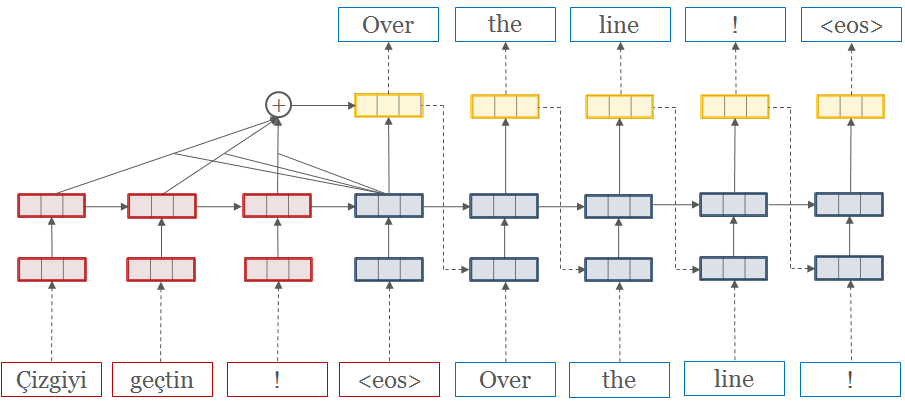
\includegraphics[width=\linewidth]{simple-attn}
  \caption{Schematic view of neural machine translation. The \textcolor{red}{red} source words are first mapped to word vectors and then fed into a recurrent neural network (RNN). Upon seeing the $\langle$eos$\rangle$ symbol, the final time step initializes a target \textcolor{blue}{blue} RNN. At each target time step, \textit{attention} is applied over the source RNN and combined with the current hidden state to produce a prediction $p(w_t| w_{1: t-1}, x)$ of the next word. This prediction is then fed back into the target RNN.}
\end{figure}


% \begin{itemize}
% \item One column describing the technical details
% \end{itemize}

\section{Implementation}


OpenNMT is a complete system and library for learning, training, and
deploying neural machine translation models. The system is successor to
the \textit{seq2seq-attn} system developed at Harvard, using roughly
the same external interface, but with a complete rewrite of the
internals to ease readability and generalizability. 

The system is implemented using the Torch mathematical framework and
neural network library, and can be easily be extended using Torch's
internal standard neural network components. Originally, external RNN
components libraries were used, but the current version uses its own
RNN implementation for fine-grained control of memory allocation. The
training aspects of the library are highly tuned for single or
multi-GPU usage. The test component can be run either on CPU or GPU, and uses batched beam search to speed up the translation process.

The system has been developed fully as an open-source project on GitHub at \url{http://github.com/opennmt/opennmt} with most contributions coming from Systran and, across the ocean,  the Harvard NLP group. Since official beta release, the project has been starred by over 500 users, and there have been active development by those outside of these two organtizations. 

One nice aspect of the implementation is its relative compactness. The complete OpenNMT system including preprocessing is roughly 4K lines of code. For comparison the Moses SMT framework including language modeling is over 100K lines.   



\section{Design Goals}

As there are now many descriptions and details of low-level RNN and beam search implementations, we skip many of these details and instead focus on the main design desiderata that motivated OpenNMT: efficiency, modularity, and extensibility. 
We point interested readers to the code for implementation notes.  

\subsection{Efficiency Optimizations}

As NMT systems can take from days to weeks to train, training
efficiency is a paramount research concern. Slightly faster training
can make be the difference between plausible and impossible experiments. 

\paragraph{Memory Sharing}

With some exception standard consumer GPUs are currently limited to 12
GB of memory. When training NMT models, the memory size limits the
plausible batch size of the system, and thus directly impacts training
time of the system. Neural network toolkits, such as Torch, are often
designed to trade-off extra memory allocations for speed and
declarative simplicity. For OpenNMT, we wanted to have it both ways,
and so we implemented an external memory sharing system that exploits
the known time-series control flow of NMT systems and aggressively
shares the internal buffers. This makes the system slightly less
flexible than toolkits such as Element-RNN \cite{}, but provides a
saving of almost 70\% of GPU memory. This in turn allows for much
larger batch sizes.


\paragraph{Multi-GPU} OpenNMT additionally supports basic multi-GPU
training. The implementation is relatively straightforward, each GPU
runs its own instance of the model. We run async SGD


\paragraph{C/Mobile/GPU Decoders} During training NMT systems require
signficant code complexity and storage to implement backpropagation
through time and parameter updates. At test time the system is much
less complex, and only requires forwarding values through the network
and running a beam search that is much simplified compared to SMT. To
exploit this, OpenNMT includes several different decoders optimized
for different environments: a batched GPU decoder for very quickly
translating a large set of sentences, a simple single-instance decoder
for use on mobile devices, and a specialized C decoder. The last
decoder is particularly useful for industial use as it can run on CPU
in standard production environments. The decoder reads the structure
of the network from Lua and then uses the Eigen package to implement
the basic linear algebra necessary for decoding.




\subsection{Structural Modularity}

While training efficiency was a primary concern, this goal was
balanced with the desire to keep the code readable and modifiable by
an advance undergraduate.  We targeted this goal by explicitly
separating out the above optimizations from the core model, and by 
documenting each module with mathematical diagrams describing how 
it connects to the underlying neural network descriptions. To test whether 
this approach would allow novel feature development we experimented with 
two case studies. 

\paragraph{Case Study: Factored Neural Translation}

In factored neural translation models \cite{}, instead of simply
generating a word at each time step, the model generates a word and
its features. For instance, the model might have a separate case
feature, in which case it would model the probability of the
lower-cased word form and the case marker. This extension requires
modifying both the output of the decoder to generate multiple symbols,
and also the input to the decoder to take in a word and its features.

In OpenNMT both of these aspects are abstracted from the core
translation code, and therefore we were able to add factored
translation by modifying the input network to instead process the
feature-based representation, and the output generator network to
instead produce multiple conditionally independent predictions.  This
option can be turned on by modifying the training data to include the
factored words.


\paragraph{Case Study: Variant Attention}

The use of attention over the encoder at each step of translation is
crucial for the model to perform well. The default method is to
utilize the gloabl attention mechanism proposed by \cite{}. However
there are many other times of attention that have recently proposed
including local attention \cite{}, sparse max attention \cite{},
heirarichical attention \cite{} among others. As this is simply a
module in OpenNMT it can easily be substituted. 

Recently the Harvard NLP group developed a new method known as
structured attention \cite{}, that utilizes graphical model inference
to compute this attention. The method was quite involved and required
custom CUDA code to compute efficiently. However the method is
modularized to fit the Torch NN interface and can therefore be
directly used in OpenNMT to substitute for standard attention.


\subsection{Extensibility}

The last goal of OpenNMT is to realize the deep learning is a very
quick moving area and that likely within the next couple years there
will be many unexpected applications of these style of
methods. Already we see related, but very different work in
variational seq2seq auto-encoders \cite{}, one-shot learning \cite{},
and neural turing machines \cite{}. 


\paragraph{Image-to-Text}

As a final case study, we experimented with implementing a complete
image-to-text translation system using the OpenNMT
library. Qualitatively this is a very different problem than standard
machine translation as the source sentence has a different modality.
However, it seems like the future of translation may require this
style of multi-modal inputs \cite{}. In particular, we adapted the
im2markup system developed by \cite{} to instead use this library.
Instead using word embeddings, this model requires a deep convolution
over the source input. However as this part of the network is
pluggable, it could be naturally defined in Torch. In fact, excepting
preprocessing, the entire adaptation requires only 500 lines of code and 
is open sourced as \url{github.com/opennmt/im2text} 


\section{Benchmarks}

Mainly focus on NMT. Speed, memory, accuracy. 

\begin{table}
  \centering
  
  \caption{Performance Results. Several languages}
\end{table}


\begin{table}
  \centering
  
  \caption{Speed Results. Multi-GPU, distillation, c decoder}
\end{table}

Picture of demo application running 

\section{Conclusion}


\bibliography{writeup}
\bibliographystyle{eacl2017}


\end{document}
